\documentclass[12pt, a4paper]{article}
\usepackage[UTF8]{ctex}
\usepackage{amsmath}
\usepackage{amssymb}
\usepackage{amsthm}
\usepackage{geometry}
\usepackage{enumitem}
\usepackage{indentfirst}
\usepackage{caption}
\usepackage{fancyhdr}
\usepackage{booktabs}
\usepackage{titlesec}
\usepackage{draftwatermark}%水印
\usepackage{graphicx} % 导入图像的宏包、单图
% 页面布局设置
\geometry{top=2.54cm, bottom=2.54cm, left=3.18cm, right=3.18cm}

\SetWatermarkText{B站：布加拉提}
\SetWatermarkScale{0.4}

% 行距设置
\linespread{1.5}

% 段落设置
\setlength{\parindent}{2em}
\setlength{\parskip}{0.5em}

% 节标题格式设置
\titleformat{\section}{\normalfont\Large\bfseries}{第\chinese{section}章、}{1em}{}
\titlespacing{\section}{0pt}{2.5ex plus 1ex minus .2ex}{1.3ex plus .2ex}

% 定理环境设置
\newtheoremstyle{solution}
{}
{}
{}
{}
{\bfseries}
{、}
{1em}
{}
\theoremstyle{solution}
\newtheorem{sol}{解}

% 页眉页脚设置
\pagestyle{fancy}
\fancyhf{}
\fancyhead[C]{b站布加拉提整理（回忆版）b站甘茶w独家讲解}
\fancyfoot[C]{\thepage}

\rfoot{整理人：八方\\资源提供：考研乔瑟夫}
\lhead{
\includegraphics[width=0.06\linewidth]{p1.png}}
\rhead{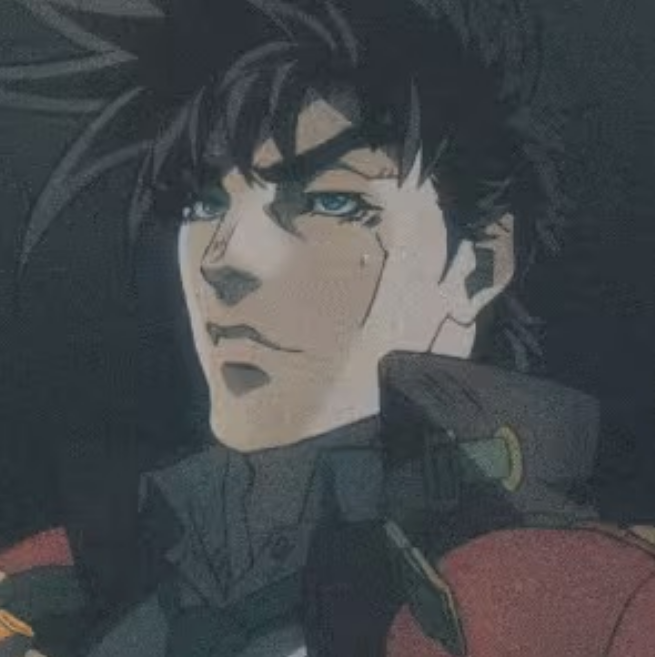
\includegraphics[width=0.06\linewidth]{p2.png}}
\renewcommand{\headrulewidth}{0.4pt}
\renewcommand{\footrulewidth}{0.4pt}

\begin{document}

\begin{center}
\Large\textbf{2021哈工大硕士考试试题：805物理光学}
\end{center}





\section*{一、填空题（20分）}
\begin{enumerate}
    \item 麦克斯韦方程组里两个最基本的物理量是\_\_\_\_\_，\_\_\_\_\_。
    \item 惠更斯提出了\_\_\_\_\_概念，后菲涅尔引入了\_\_\_\_\_，优化了惠更斯理论（模糊）
    \item 平面电磁波传播过程中电场强度与磁场强度是\_\_\_\_\_关系，电场强度与磁感1强度是\_\_\_\_\_关系。
    \item $E=6(2\pi (0.5x-4t))$，这束光的频率，波长，振幅，相速度，传播方向分别是\_\_\_\_\_，\_\_\_\_\_，\_\_\_\_\_，\_\_\_\_\_，\_\_\_\_\_。
    \item 光从一个介质进入到另一个介质，电场\_\_\_\_\_分量连续，磁场\_\_\_\_\_分量连续。
    \item 反常色散的光谱曲线中折射率\_\_\_\_\_，正常色散的光谱曲线中折射率\_\_\_\_\_。
    \item 两个频率相同，振动方向相同，而传播方向相反的单色光波叠加，产生相邻的两个波节之间的距离为\_\_\_\_\_。
    \item 光线在与介质表面相互作用时，设计到的物质方程有\_\_\_\_\_，\_\_\_\_\_，\_\_\_\_\_。
\end{enumerate}
\section*{二、名词解释}
\begin{enumerate}
    \item 瑞利判据
    \item 倏逝波
    \item 偏振度
    \item 光栅
    \item 折射定律
    \item 电光效应
    \item 条纹对比度
\end{enumerate}
\section*{三、选择题（单选加多选）}
\begin{enumerate}
    \item 相同孔径的微博望远镜和可见光望远镜，为什么微波望远镜比可见光望远镜分辨能力差？（选项丢失）
    \item 入射角大于临界角，且入射线偏振光振动与入射面交角非0度或90度，反射光是什么？
    A.线偏光\quad B.椭圆偏振光\quad C.自然光\quad D.部分偏振光
    \item 下列不能作为偏振元件的是（选项丢失）
    \item 如何提高显微镜分辨本领？
    A.增大波长\quad B.减小透镜焦距\quad C.减小波长\quad D.油浸透镜
    \item 填空看起来是蓝色的，是什么原因造成的？
    A.大气中光的折射\quad B.大气中光的反射\quad C.大气中光的衍射\quad D.大气中光的散射
    \item 将矩形孔的弗朗合费衍射实验装置中的矩形向一侧平行移动，衍射图样会发生什么变化？
    A.衍射图样按照同样方向移动\quad B.衍射图样暗反方向移动\quad C.衍射图样没有任何变化\quad D.无法确定
    \item 线偏振光经过半波片变成什么光？
    A.线偏振光\quad B.圆偏振光\quad C.部分偏振光\quad D.无法确定
\end{enumerate}
\section*{四、简答题}
\begin{enumerate}
    \item 简述空间相干性和时间相干性的定义，以及二者由和产生
    \item 由点光源获得相干光的方法有哪些？并举例说明相应的装置，的波面干涉和分振幅干涉分别涉及什么原理？典型干涉装置是什么？
    \item 相机物镜和望远镜的分辨本领由什么决定？如何提高二者的分辨本领？
    \item 简述线偏振光和自然光的异同
    \item 什么是旋光效应？法拉第旋光效应与自然光旋光效应有什么异同？
    \item 什么是等倾干涉？其干涉条纹有什么特点？
    \item 简述瑞利散射的特点
    \item 简述有哪些获得偏振光的方向？
\end{enumerate}
\section*{五、计算题}
\begin{enumerate}
    \item 太阳光30度入射双层玻璃$n=1.5$，求折射率，偏振度
    \item 空气劈尖等厚干涉，劈尖夹角$2\times10^{-4}rad$入射光波长$450nm$，注入$n=1.4$的液体，求液体注入前后第五级亮纹分别移动了多少距离。（全求出来，问的有问题）
    \item 平行平板等倾干涉装置，望远镜的观测角为6度，入射光波长$500nm$，平板厚度$h=3mm$,中心是亮还是暗，为什么？望远镜能观察多少条亮纹？
    \item 波长$500nm$激光，通过$0.0025mm$的狭缝，透过焦距$50nm$（模糊）的透镜汇聚到焦平面，求第一级亮纹和第二级亮纹距离焦平面中心的位置。若中心光强为$I_0$,求第一级亮纹和第二级亮纹的光强？
    \item 一束部分偏振光，光强最大方向是$I_0$,偏振片旋转$\pi/3$,光强变为一半，求偏振度。 
\end{enumerate}
\section*{六、论述题}
\begin{enumerate}
    \item 如图，在某接近理想系统成像系统的光学系统中，加入挡光版A，其圆心在光轴上，用物理光学理论分析其对成像系统的影响。
         \begin{figure}[!htb]
                \centering
                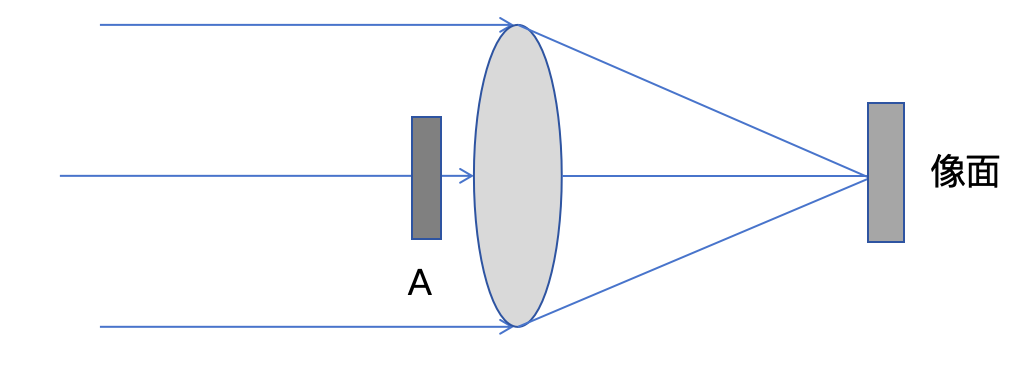
\includegraphics[width=0.7\linewidth]{211.png}
                
          \end{figure}
\end{enumerate}
\end{document}